\section{Results} \label{results}
% \subsection{Activity in the wild}
% \subsection{Light levels in the temperate forest}

\subsection{Wild \textit{Nebria brevicollis} rest during the day}
We compared the mean activity during day and night under LD conditions in the laboratory. We find that wild \textit{Nebria brevicollis} rest during day and show higher activity levels during night (Paired t-test, n = 34, mean of the differences = -0.09, 95\% CI [-0.11, -0.07], t(38) = -7.68, p < .001; Cohen's d = -1.23, 95\% CI [-1.66, -0.82], Fig. \ref{fig:activity-all-individual}, Fig. \ref{fig:activity-all}). 

% They are able to maintain their circadian rhythm under LL conditions, potentially slightly accelerated.

\subsection{Increased activity levels during with light present}
We then went on to compare different light conditions with a mixed effects model. We used stepwise model selection using Akaike's Information Criterion (AIC) (Table \ref{tab:model-summary}A). The model selection found no effect of sex, which was left out of the final model. We find that the difference in activity for day and night (time of day) exists across all light conditions (Table \ref{tab:model-summary}B). However, we also find interaction effects between time of day and light conditions. These interactions only appear for night, with no interactions on day-time activity. LL increases activity during the night, whereas DD decreases activity (Table \ref{tab:model-summary}B).

\begin{figure}
    \begin{fullwidth}
        \centering
        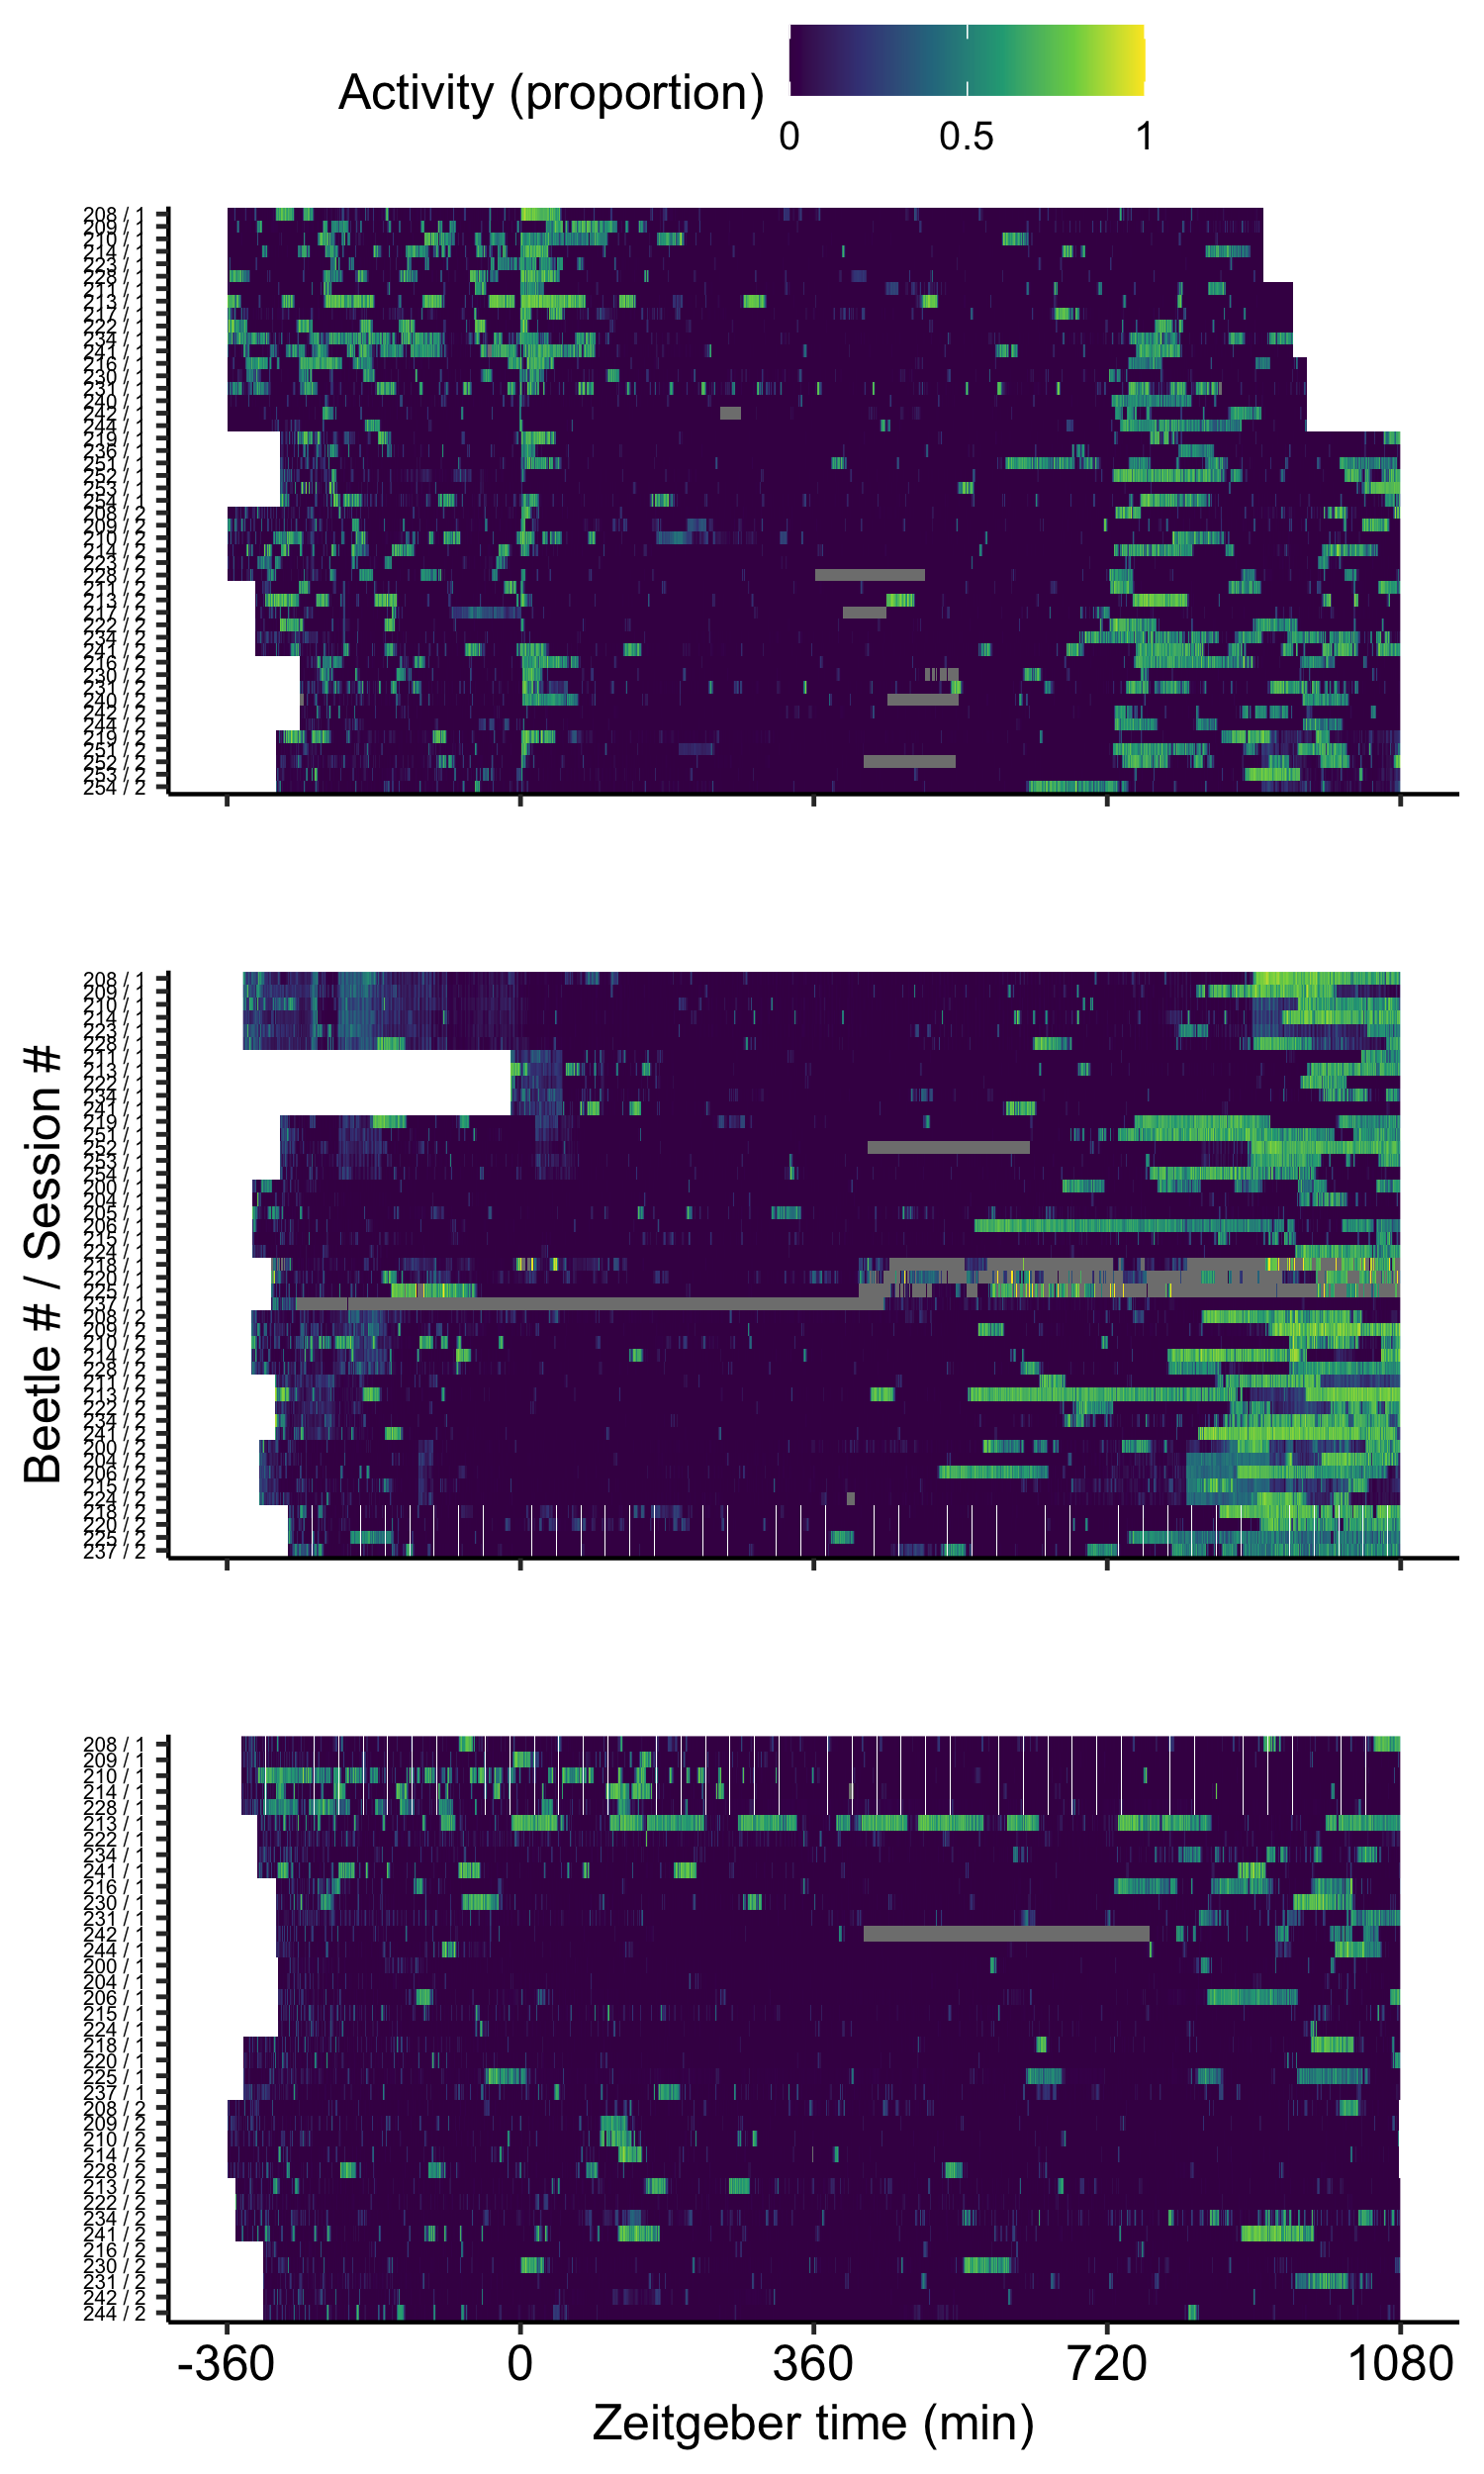
\includegraphics[width = 0.9\hsize]{src/figures/all-individual-activity.png}
        \caption{Raw data for all experiments across all conditions. Each row is a 24 hour trial, with time along the x-axis. Colour corresponds to the time spent active per minute from 0-1. Top) LD condition. Middle) LL condition. Bottom) DD.}
        \label{fig:activity-all-individual}
    \end{fullwidth}
\end{figure}

\begin{figure}
\centering
    \begin{subfigure}{\linewidth}
        \caption{}
        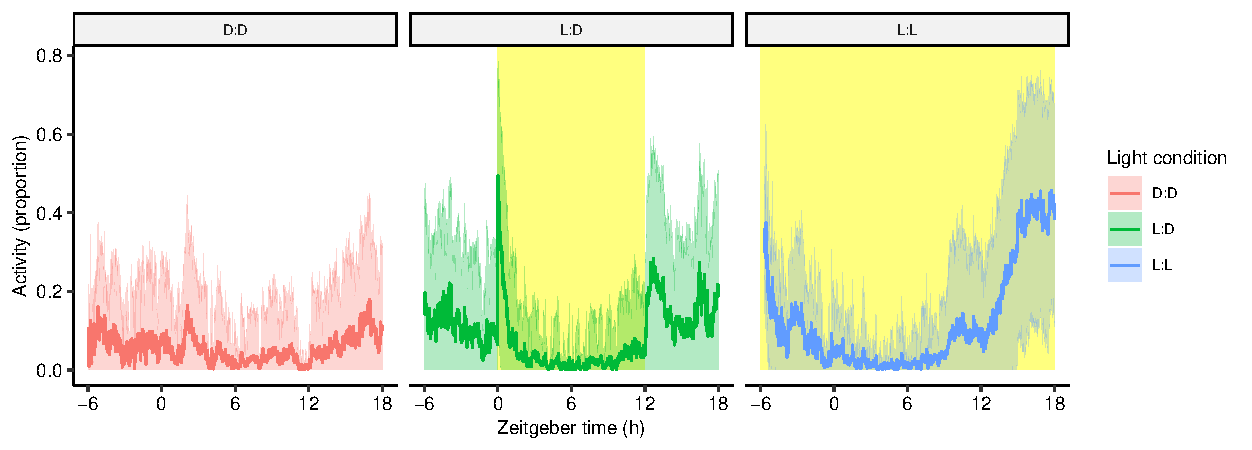
\includegraphics[width = \hsize]{src/figures/activity-all.pdf}
        \label{subfig:activity-all}
    \end{subfigure}

    \begin{subfigure}{\linewidth}
        \caption{}
        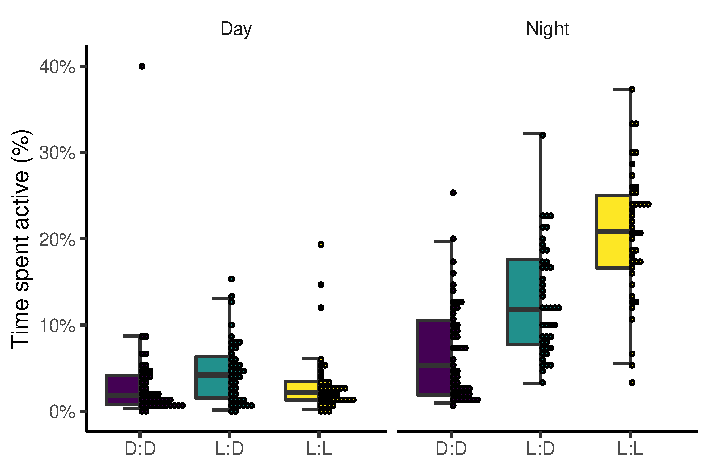
\includegraphics[width = \hsize]{src/figures/night-day.pdf}
        \label{subfig:night-day}
    \end{subfigure}

    \caption{Activity of \textit{Nebria brevicollis} depends on light conditions. A) Proportion of time spent active during 24 hours. Lines indicate mean activity \textpm SD across all beetles. Yellow boxes indicate lights are on. B) Time spent active across light conditions and sexes. Boxplots show median, 25th and 75th percentile and highest and lowest value within 1.5$\times$IQR. Dots are each individual observation. Activity during the night increases in LL and decreases in DD, irrespective of sex, whereas daytime activity is unaffected (Table \ref{tab:model-summary}).}
    \label{fig:activity-all}
\end{figure}

\subsection{Abrupt changes in light intensity}
\textit{The LD data suggests that effects of onset and offset of light have great impacts on activity, though with different time constants.
I have not had time to do the proper analysis for this yet. Additionally, it will be interesting to see what happens with a gradual light change. I have yet to perform the experiments with gradual light changes, but will also be doing those within the coming month.}

